%
% The first command in your LaTeX source must be the \documentclass command.
\documentclass[sigchi]{article}
% The first command in your LaTeX source must be the \documentclass command.
\usepackage[English]{babel}
\usepackage{tocloft}
\usepackage{pdfpages}

\def\BibTeX{{\rm B\kern-.05em{\sc i\kern-.025em b}\kern-.08emT\kern-.1667em\lower.7ex\hbox{E}\kern-.125emX}}
\addto\captionsEnglish{
    \renewcommand{\contentsname}%
    {\huge INDEX}
}


\pagenumbering{gobble}% remove page count

\begin{document}
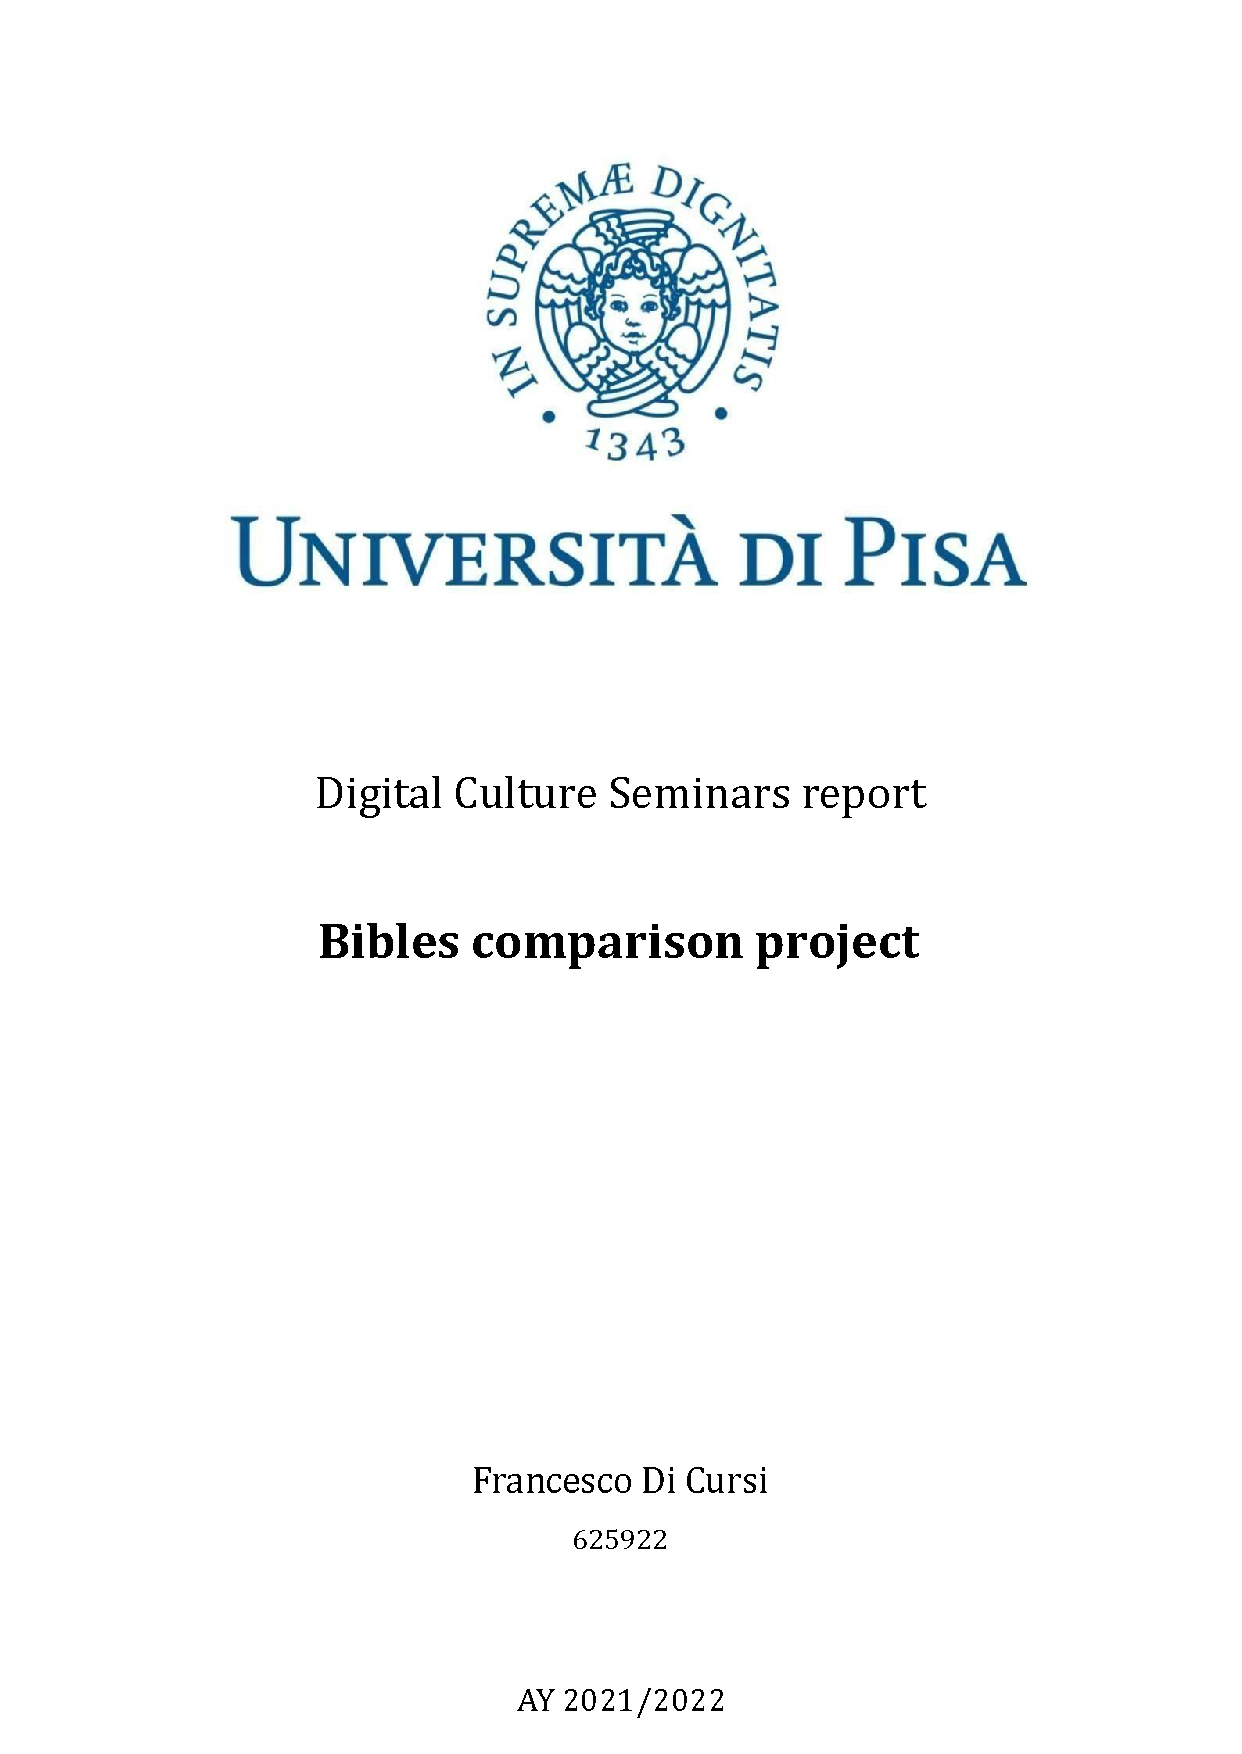
\includepdf[pages=-,pagecommand={},width=\textwidth]{Copertina_finaleTA.pdf}

%remove references
%\settopmatter{printacmref=false}
%\setcopyright{none}
\renewcommand\footnotetextcopyrightpermission[1]{}
\pagestyle{plain}
%replaces \tableofcontets and stops self reference in toc
\makeatletter
\begin{a}*
\centering
\tableofcontents
\end{a}


% This command processes the author and affiliation and title information and builds
% the first part of the formatted document.
% WITHOUT THIS LINE DOUBLE COLUMN DOESN'T WORK

\maketitle
\pagenumbering{arabic} %restart page count from introductionS
\begin{abstract}
    The present work aims at exploring different versions of the bible in order to spot major differences according to different \textit{faith groups}. This is done by looking at the parataxis/hypotaxis distinction (to highlight changes in the text structure) and the co-occurrence of both entities-entities and entities-common nouns (along with their sentiment). The usage of tokens and trigrams is also inspected. This prototypical tool is conceived to be scalable and has no predetermined target: it is useful as long as the user is curious to explore. Finally, it is an open-posed problem which can yield a complete answer on extensive search. Here an example is provided to guide the user, leading to the conclusion that, if compared to a strongly literal translation (Young's Literal Translation), the Jehovah's Witnesses translation (New World Translation) results heavily manipulated both in terms of structure and characters.   \\ \\

		\textbf{\textit{Keywords}}: \textit{Bible; Comparison; Writing style; Characters; Text manipulation}

\end{abstract}
\section*{Introduction}
\addcontentsline{toc}{section}{Introduction}
The idea of the present seminal work stems from “The Visual Agency” project about Dante \cite{dante}. In their project it’s possible to explore the Divine Comedy in its structure and contents using smart visualizations that allow to convey complex information in a simple glance. Their actualization tools are mainly \textbf{Vue js framework} and \textbf{d3.js library}.
The main problem in realizing a similar tool has been the impossibility of replicating the multimedia richness of the site (due to the lack of authorizations) and the lack of a whole team made up by expert designers.
In these terms, the present work drifts from the original idea in that the focus goes essentially to the structure of the chosen text: the Bible. In order to keep somehow the complexity of the Visual Agency’s project, the decision to compare different versions of the Bible has been made, in the attempt to answer to different questions which will be presented soon.
The Bible has been chosen as the target book (better, ensemble of books) because of different reasons:
\begin{itemize}
    \item it is probably the most sold and translated book of all the time (w.r.t non-fiction books, a possibly not universal classification);
\item it shaped western society from inside (it is the very basis of the idea of Euorpe as omnia catholicorum, as a common shield towards the Ottoman expansion in 1400) ,  and it has also been the ideology weapon allowing the western culture to colonize, both physically and mentally, the entire world;
\item it is probably one of the best indexed text, as any part of it is retrievable by the “Book chapter:verse” pattern by default, in each of its version;
\item given the statement in point 1, there are many different digital libraries which propose plenty of its versions for free;
\item personally, even if it is the cultural basis of the West, still it is a cultural misappropriation as the proper owners of the Old Testament are Jews and it is, probably and by the perspective of the borrowers, a set of books lost in theology and translations.
\end{itemize}

These and other reasons then led to the following questions, in an attempt to produce a visual analytics tool which seems not to be produced by anyone else:
\begin{enumerate}
    \item being the Bible born in an oral tradition  and being constantly manipulated both orally and chirographically across the millennia from different traditions, 
how much of the orality-like structure (i.e. parataxis)  is preserved? And conversely: how much the written style (i.e. hypotaxis) has filled these pages?
\item Is the communication style related to the length of the verses?
\item What are the most used tokens?
\item What are the most used trigrams and how are they distributed in text?
\item What relations hold between entities in text? What’s the sentiment associated with both entities and the context in which they co-occur?
\item What relations holds between entities and concepts?
\end{enumerate}


An interactive tool has been produced to try to address these problems, in a human-friendly approach (i.e visually, rather than using just raw computations).
Finally, as a disclaimer, this prototypical work is brought up by a non-expert in the Bible field and it aims at posing an open question and not at giving a resolute response. This open question is posed free by any religious preference but with the clear presupposition that something that is taken from different cultures translates, not only linguistically, to something else: to something that is accessible to the hosting culture, translating unfamiliar shapes and nuances to familiar ones, either for the sake of clarity or ideology coherence.


\section{Work flow and implementation choices}
The workflow of the present project is the following:
\begin{enumerate}
   \item searching for a digital source giving free access to different bible versions;
   \item web scraping and data preprocessing;
   \item realization of an interactive visual analytic tool to address the questions posed in the introduction.
\end{enumerate}
The search for a suitable source and the scraping/preprocessing phase will be covered together, as it has been a trial and error driven phase. \\ \\

1 \& 2. Even if there are, as already said, plenty of digital archives giving access to bible versions, the search for a suitable source has been quite time consuming. The idea of the work started from a bible database called \textbf{eBible} \cite{ebible} due to its completeness (in both resources and descriptions). Python has been used as language to create a scraping script with \textbf{Selenium} \cite{selenium} (a powerful python library creating an instance of the browser on which to replicate surfing user behaviour). After all English versions were gathered (see ‘scraping bibles.py’), another Python script has been created in order to convert pdf files to csvs (see ‘pdf to csv (only one column).py’). This first approach has proven not to be the ideal one as the Occam’s razor would suggest: retrieving the text from a pdf (with no structured text basically) is way more risky than retrieving it from a plain html (highly structured by nature). In the case of pdf, the “pdf to csv” script has been implemented  only for the one columned layout (for sake of simplicity) leading to ignore many English versions present on the site. Moreover, even if these texts are structurally standardized, they tend to diverge in some aspects: unstandardized annotation signs, presence/absence of notes as footers, arbitrary use of digits or natural words to indicate integers (eg. “10 men”), etc… .Although the implemented script shows the attempt to overcome these and other problems, the choice has been that of changing approach, also to reduce the number of versions to a more feasible number and with an higher reliability. Between the many online archives, \textbf{Bible.com} \cite{biblecom} has been chosen, given its minimal and comfortable design as well as its richness of resources. So again, a new scraping script has been realized ad hoc for the site with the same methodology as the previous attempt, this time leading to a more desirable result. From this site, the following versions have been downloaded:
\begin{itemize}
    \item Orthodox Jewish Bible: chosen due to the integrity of jewish expressions, left untranslated as  “ [...] it applies Yiddish and Hasidic cultural expressions to the Messianic Bible” \cite{OJB}. This version has been retained even if problematic w.r.t proper nouns and sentiment identification (a task that will be described further);
    \item Young’s Literal Translation: chosen as it is  “ [...] an extremely literal translation that attempts to preserve the tense and word usage as found in the original Greek and Hebrew writings” \cite{YLT};
    \item New World Translation: the Jehovah’s Witnesses Bible;
    \item New Revised Standard Version: ecumenical version made by  the National Council of Churches which is accepted by many Protestant, Catholics and Orthodox churches (even if from this version stem different specified versions according to each church) \cite{NRSV}.
\end{itemize}



This scraping has been conducted with the “New scraping.py” file. Regex has been used in order to treat some errors in retrieving: some verses weren’t splitted (yielding to a verse made up by more than a verse). There were verses having the verse index splitted by a space (e.g. 1 2): in this case the regex / \verb/(^\d+)(\D+)(\d+\D+)/ / has been used in order to remove the second group (the non digits characters, being mostly the space). Other verses (“internal” verses in not correctly splitted scenario) had a special character “ ‘ “  after the index: in this case the
 / \verb/(^\d+)(\‘)(\D+)/ / pattern has been used to, in a similar fashion as in the previous regex pattern (removing the second group). Then, to overcome the problem of internal wrong split (e.g. 1 Verse2 Verse3… ;) the following regex pattern has been used / \verb/(\d+\s\D+)(\d+\D+)/ / where the first group is the sentence starting with and index, followed by a sentence starting with another index but with no space after. This regex gave all verses but the last one, so another pattern has been used to separate also this one (i.e.  / \verb/(\d+\s?\D+)$/ / ).
The result had duplicate verses (not actually identical given the presence of characters as the square bracket and others) so, before saving the csv, the .drop\_duplicates command of pandas library has been used on the subset “Book, Chapter, Verse\_idx”, in order to drop records having same book, chapter and verse index. The script works by scraping each and every book of the version, saving each book as a different csv (being a time consuming process, this approach ensures to save data in case of some errors). Finally, this script has two “stances”: one for those texts without the above mentioned problem treated with regex, and another for those that do have the problem (case that has been described above). By the way, all the books in all the versions had this problem, as the output of the function suggests (‘correcting’ appears in the output if the regex detects the pattern, otherwise it simply saves the result).

The next step has been concatenating the retrieved books in a single dataframe. There were still unwanted records (those starting without a digit, as the name of chapter or some inline notes) so again, a simple / \verb/^\D/ / regex pattern has been the way to clean the dataframe in this case. Finally, all the names of the books for all the versions have been standardized using the Young’s Literal Translation books as keys in a dictionary. This could be a problematic approach, since there is the loss of the information on the name of the book but this is not particularly relevant in this work as long as these books are actually the same conceptually (eg. “Genesis” in Young’s Version; “Bereshit” in Orthodox Version)

The concatenated dataset at this point consists of 4 columns: Edition, Book, Chapter, Verse. It was ready to be fed into the visualization tool but, for a further analysis, some new features were added: the Sentiment, the Summary and the Proper Nouns, together with Subjectiveness which at the end has not been used to not over complicate the visualizations.

The task has been conducted with \textbf{Spacy} \cite{spacy} at first (an high-level NLP python library) starting with the search for proper nouns ( choosing the ‘PROPN’ pos attribute for each of the retrieved tokens). Then, realizing that it was a too powerful tool for this work,  the choice to use another, simpler, NLP library (i.e. \textbf{textblob} \cite{textblob}) has been made. By continuing with textblob, the ‘sentiment\_assessments’ built-in function to calculate “polarity” (i.e sentiment, -1 for highly negative to +1 for highly positive) and  “subjectivity” (from 0 for objective to 1 to subjective). The “Summary” dimension has been produced by looking for ‘NN’ pos for each of the token in the verse and by taking its lemma (using textblob ‘.lemmatize()’ function), yielding to a list of common nouns giving an idea of the content of the verse. These words are ordered by their frequency, as for the names in Proper Nouns.
These new columns were then added to the previous concatenated dataframe.

After this, there were still errors in both proper nouns and summaries:
‘titled’ common words were found in proper nouns (e.g. Day, Night, etc…) and ‘hill-retrieved’ words (eg. [the) were present in summaries.
To overcome the proper nouns problem, the “English\_words” library has been used as a dictionary, in order to filter out the common words from the proper nouns. It must be mentioned that “god” as well as “spirit” and other relevant words were present but, in order to not to adhere strictly to theology assumptions, only God has been retained as entity, while discarding words as spirit (the information is not loss as these nouns are present in the “Summary” dimension). Here, the Word module from textblob library (allowing for single word analysis) has been used to lemmatize each of the names in order to compare it with the English dictionary (eg. $Heavens \rightarrow heaven; Went \rightarrow go $ ; …). The resulting list is, partially, the correct list of proper nouns (terms as "beloved" are not present in dictionary and the lemmatizer can't treat them correctly).
In the case of summary, on the other hand, the idea has been to remove not alphabetical tokens.
As a side discours, besides ‘Spacy’ and ‘textblob’,  other libraries to perform NLP in python are \textbf{nltk} \cite{nltk} (a powerful yet low-level library born as a didactical tool) and \textbf{Gensim} \cite{gensim}  but these two libraries are used more in machine learning applied to text, and that’s not the aim of this work. \\ \\

3. The visual tool has been implemented using javascript, more precisely the Vue 2 framework. The older version of the framework has been used because of the stability of \textbf{BootsrapVue} \cite{bootstrapvue}, a handy wrapper allowing to easly use Bootstrap in Vue framework. Among all things, it offers the b-container tag that helps in the disposition of elements in the page (using b-columns and b-rows) in a responsive fashion. Vue has also been used, as already mentioned, to stick with the methodology of the chosen seminar. In general, the framework choice in js is relatively arbitrary as any framework allows to reach the same result but using different methods. In this case, \textbf{Vue Options API} \cite{vueapi} logic offers an intuitive lifecycle hook compared to the \textbf{React one} \cite{reactapi} but, again, it’s a personal preference led mostly by habit. Frameworks, obviously, are useful yet not mandatory.

The web app is composed of different sections handled by using \textbf{conditional rendering} (v-if) \cite{vueconditional}. This method is \textbf{usually criticized} \cite{vuewarning} as there are better alternatives, in particular case with a higher number of components (in which the “forceUpdate” or the “key” approach would be more suitable) but in this case, having just two components, the conditional rendering is an acceptable approach.

The main idea was that to display all the informations of all the versions in a single page but it would have been computationally expansive, leading to potential lag due to the high number of plots. To overcome this problem, two different sections have been created: single section and binary section.
The single section allows the in-depth inspection of a single version through a set of plots; the binary one can be used to compare 2 versions verse by verse (in this section plotting has been reduced to the essential).
Another problem, w.r.t the first section, is that of the impossibility to display the whole bible (again, for a performance sake) so the default and suggested option is that to visualize book by book rather than the whole bible. Still, the user is free to choose “All” in book selector, selecting thus all the books of a given version, but leading almost certainly to a browser crash. The user with a reasonably good machine could succeed in visualize all the books but he would have to await a considerable amount of time.

The first section is composed by a set of global handlers in which the selection can be made according to “Version”, “Book”, “Chapter” and “Verse” (white, red, green and blue selectors). This handler communicates to be global as its position is fixed and follows the user scroll. The user is also free to hide this by using the “Hide”/”Show” toggle positioned at its side. 

Before going further with the page description, the main idea of exploring the writing style has been realized in a simple fashion: conjunctions are a clear sign of the complexity of a sentence where coordinating conjunctions lead to a simpler structure than the subordinating ones. A problem is that listing the coordinating conjunctions (i.e. "for", "and", "but", "nor", "or", "yet", "so" ) is easier than listing the subordinating ones, so the most common of them has been used (being almost 60, look for “subord\_conj” variable in  “Single\_section.vue” component). Obviously, this is the simplest approach as a further implementation would also use other important elements of the discourse as punctuation (e.g. where comma and semicolon could be signs of juxtaposition, an orality-like structure) or narration stratagems (e.g. using a personal way of writing as in “I believe that…” for an orality-like case or an impersonal way as in “It is believed that… ” conveying the so-called “objectifying masking”, giving a sense of detachment and formality). These and other elements would be added to the computation in a possible further implementation of the web app. Finally, the actual implementation of the function changes according to the context in which it has been used (i.e. whole verses, tokens or trigrams). More on this will be said further, while describing each plot.


\section{Single section}
Plots have been realized with Plotly.js, the javascript version of the popular python library. This has been done to not reinvent the wheel as well as it is a highly interactive library, perfectly suitable for this project. Where actually needed, as it will be explained in the case of the network visualization, a lower level library has been used (i.e. d3.js) to implement a more customed and complex visualization.
\subsection{Verse viewer}
In the verse viewer, all the verses of the selection are displayed. Their color is conditioned on the number of the types of the conjunctions appearing in them: a blue verse is a mostly hypotactic (i.e. with subordinating conjunctions), a gray one is neutral (no conjunctions or an equal number of subordinating and coordinating ones) and a red one is mostly paratactic (i.e. with coordinating conjunctions). For each verse, first an absolute count of the conjunctions is made, where coordinating conjunctions accounts for +1 and subordinating ones for -1 (so analyzing the verse token by token, checking for the type of the conjunction). For each type a different list is created so that each of the elements of the list accounts for a verse, where the position of the element in the list is the index of the verse. At the end the two lists are summed leading to a new list of the same length but with each element being the result of the sum of the occurrence of the two types of conjunctions (eg [5,..] states that the verse one has 5 coordinating conjunctions while [-3,...] states that the same verse has 3 subordinating conjunctions, so the result would be [2,...]. If the result is higher than 0 then the verse is mostly paratactic, if it is 0 then it’s neutral and if it is lower than 0 then it’s mostly hypotactic.
At the left of the verse, the numbers explicits the book, the chapter and the verse index (following the same colors of the selectors).
\subsection{Horizontal bar chart}
Besides counting the number of verses in the title, the \textbf{bar chart} \cite{hbar} represents the percentage of each verse type. The absolute count for each category is displayed in the legend of the plot. This could be also made using a pie chart but a bar representation has been preferred as the length is more understandable as measure than degrees.
\subsection{Parallel Categories Diagram}
\textbf{Parallel categories diagram} \cite{catplot} has been used to display the same information of the bar but in a more refined way: if the bar shows the overall percentage of the entire selection, the parallel categories diagram shows this both for chapter and verses. A further element of inspection in this plot is the length of the verse, so that writing style can be compared to the length of each verse. By hovering over this plot’s elements, further informations can be seen. By hovering on the parallel axis, the displayed count is the number of all the words in the chapter (either on the chapter axis at left or the verse axis on the right). The important thing on axis hovering is the conditional probability: 
P( x $|$ color) represents how much of a given color a certain verse/book actually is (i.e. the “global” probability of a certain color being represented by the x), while P ( color $|$ x ) represents how much of the given x element is made by a certain color (i.e. the “local” probability of the color on that very element). With this in mind, this tool is useful to understand the chapter style according to each verse.
Initially the idea was that to have 4 parallel axis (Edition, Book, Chapter and Verse) but it was unfeasible due to the high number of elements on axis and the links behaviour between axis (even with a plot having just Chapter and Verse, all chapters links to the same numbers of verse leading to a meaningless and cluttered representation). In the attempt to overcome this issue, other sub div are added in the main div, in a number equal to the number of chapters selected for a given book.
In this way, even if the user has to deal with the scrolling div, the information for each chapter is easily consultable  (also with a simple glance without hovering).
This representation could be also done either with \textbf{treemap} \cite{treemap} or \textbf{sunburst} \cite{sunburst} but this hasn’t been done because both don’t allow for a clear visualization in this case: the treemap and the sunburst order elements according to dimension (thus it changes the book and verses order and it also tend to “hide” smaller elements), moreover they oblige the user to undergo a “layer representation” in which to click the element to pass to the sub-layer. The categorical parallel plot has been the trade-off between representing hierarchy but in a visually “economical space” (even if the multi sub div approach has been exploited to overcome the visualization problem mentioned above).
\subsection{Line chart}
The \textbf{line chart} \cite{linechart} has been used to represent tokens distribution according to the relative category. This plot allows to spot the frequency of conjunctions as well as neutral tokens. Given the possible high number of tokens when analyzing an entire book, 2 handlers are provided: one local handler above the plot, used to filter the plot according one of the two axis (frequency or number of tokens) and the other one in the legend of the plot (by double clicking on the category name, only that category gets highlighted). The functionality of the first handler can be replicated directly inside the plot by selecting a certain portion of space but the separate handler has been provided as it is simpler to use, as well as more precise. This plot could also have been a bar chart but a line one has been chosen as it better displays the curve of each of the three distributions (being all power law distributions). As the user can observe, the choice has  been that to use a case sensitive approach. In other words, ‘and’ and ‘And’ accounts for 2 different scenarios, being the latter a token found at the beginning of the sentence. This choice has been done as coordinating conjunctions positioned repeatedly at the beginning of a sentence are a clear sign of an oral style (they all are different sentences separated by dots, still they maintain the juxtaposition structure with high repetition, highly used in oral contexts as it helps to memorize a text).
\subsection{3D Scatter plot}
In order to display valuable informations about trigram frequency and distribution all at once, a \textbf{3D scatter plot} \cite{3Dscatter} has been used. This choice has been longly pondered as, being particularly cluttered in case of the entire book selection, can be visually hard to decode. The idea behind the choice is that a trigram is clearly a 3D pattern. Leaving the ticks on the labels ordered by occurrence (and not alphabetically or by frequency) gives a view of the actual order of the text. In this way it’s possible to spot which trigrams are used frequently since the beginning of the selection, and which are the tokens accounting for major occurrences in trigrams. In the first case, the most used trigrams are larger in size and their frequency can be seen both by hovering on the element and in the side list. In this plot x,y and z stands for first, second and third token composing the trigram. In this way it’s easier to spot the most used token in trigram (and the position in which it is used) by simply looking for a long line (given a fixed axis): the line indicates that, given a fixed dimension (e.g y, the second word of the trigram), other trigrams are formed with that token in that specific position (so in the case of y, the line is fixed on the y dimension while it progresses through x and z axis). 
Given the complexity of the plot, a set of local handlers have been realized: 
the first one is the scale selector (absolute values or scaled by the square of the value multiplied by an arbitrary constant, i.e. 5); the second one is the annotation selector (whether to show the annotations or not, consisting in most frequent trigrams according to category and the highlighting of the 0 point); the third one is the category selector (display all points or only those containing coordinating/subordinating tokens) and finally the mesh layers (whether to show the mesh layers or not).
The mesh layer is problematic if used with the entire book selection: the advice is that to use it only with chapter or verses due to possible crashes. This mesh uses the \textbf{alpha-shape algorithm} \cite{alphashapealg} (being the alphahull value greater than 0) in order to spot clusters. To enhance the power of this visualization, a mesh layer for each of the categories has been realized. This could help the user to better understand the distribution of trigrams across the text along with their type. Note that in the case of “All” in the  category selector, subordinating mesh layer is drawn on top of the others as it’s the rarest category, then there is the coordinating layer and then the most common of all, the neutral layer.
\subsection{Heatmap and Network}
In the last section of the page the user can explore both “Entity-Entity” and “Entity-concept” relations.
The former allows to inspect entities co-occurence both with a heatmap and a network visualization, while the latter only allows for a heatmap visualization. This choice has been implemented as the number of nodes would exponentially grow given the major presence of “summary words” (i.e. common nouns) if compared to entities (i.e. proper nouns). Even if a suitable way was found to represent these relationships (i.e. marking concepts with a white border, and entities with a black one), this is not always a wise choice (due to the possible lack of space). Going further with the description, while the heatmap accounts only for raw co-occurence, the network adds sentiment information both on single entities (nodes) and relative context (link). In case of nodes, their size is the frequency of occurrence of a single entity while their color varies according to the sentiment associated with that entity.
In case of links, their size accounts for the co-occurence of two entities in the same context while the colors stand for the sentiment of that very context. Values are obtained using the mean value. The used color range is [blue, lightblue, green, gray, pink, orange, red] where the relative value  mapping is [-1, -0.5, -0.25, 0, 0.25, 0.5, 1]. In this way, the most frequent entities will almost always have “neutrish” colors, oscillating between -0.25 and 0.25, and big size while rarest entities will be smaller but will mostly have vivid colors (if their context is positive or negative).
Finally, being both rendering time consuming in case of entire book selection, the plot is not drawn automatically (“Blank” option by default) in order to not slow down more the loading of the page. The user will need to manually activate this section if needed, being ready to wait in case of large selections (as the alert will suggests).
\subsubsection{Heatmap}
The \textbf{heatmap} \cite{heatmap}, as already mentioned, accounts for a raw co-occurrence matrix. In the “Entity-Entity” case, being the two axis equal, the user needs to look at half of the plot (divided by a diagonal made by the intersection of the same name, going from bottom left to top right). On the other hand, in the “Entity-concept” case, the plot is significant in its wholeness as the two axis differs (where the y axis is the set of common nouns and the x axis is the set of proper nouns). Note that, even if a strong effort has been made in order to convey only significant nouns, there can still be lesser mistakes (given the prototypicality of the project). This visualization has been chosen as it allows to easily explore the co-occurrence relationships, being the most natural visual medium for a co-occurrence matrix. As for previous plots, the order in the axis has not been ordered by any means, as the “moment of occurrence” may be significant according to the flow of events. Another important note, as previously mentioned, is that the Orthodox Jewish version contains names that are obviously hill-treated w.r.t english NLP tools. Despite this problem, this version has been retained as the user is free to search for the meaning of the terms: in this way, even if visually problematic, the user is stimulated to do a reflexive research which, hopefully, would somehow amplify his knowledge about the topic.
\subsubsection{Network}
The network visualization has been implemented using d3.js library, starting from the study of the \textbf{example given on their “Observable.com” account} \cite{networknolabel}. Another approach would have been the \textbf{hierarchical edge bundling} \cite{hieredgebundling} (i.e. a network with a circular layout) which could be more useful in case of a high number of nodes and links. An implementation of this sort will be taken into account in a possible follow-up of this project. Another visualization problem is that of node’s names: in the actual implementation, names (along with frequency and sentiment) are displayed on hover. Due to the impossibility to show node labels without hovering, \textbf{another approach} \cite{networklabel} has been attempted, yielding to the desired result.
The problem with the first attempt is that nodes are directly circle svg elements while, to easily display the node label, a g element is needed (i.e. the g element acts as a container in which to place both circles and labels). 

\section{Binary section}
This parallel section is useful to explore verse-by-verse comparison of two versions. The starting idea was that to implement further this section but, as the user can imagine, if the first section is already slow, a section with a doubled set of plots would have been unfeasible. Due to this, only the bar plot has been retained, to have an overview of the verses and their style, in order to decide previously the interesting versions and books to select in the first section. This section will be not described in the practical use.

\section{Practical case using Ruth book: YLT vs NWT}
Being the bible a particularly long text composed by several long books, a short book will be used in this circumstance due to the possible lack of space. This choice is a consequence of the list of categorical parallel plots, one for each chapter of the selection. The following example is a guide for the user in order to explain the interface usage. Note that the project is conceived to be interactive and a written report will not be exhaustive as, for example, the hovering helps in displaying valuable information (e.g. in the parallel categorical plot).\\ \\
As already mentioned, Ruth book has been chosen as it is a relatively short book (4 chapters, 85 verses in total). The choice of these two versions has been made according to the fact that the Young’s Literal Translation is a famous version in which the structure of the text (along with tenses) is preserved as more as possible (w.r.t greek and hebrew versions) while the New World Translation (the Jeova’s witnesses version) is strongly altered (e.g. certain verses are entirely omitted). Note that, from now on, acronyms will be used to address to the versions (namely YLT and NWT)
\subsection{Bar plot comparison}
\begin{figure}[!htpb]
    \centering
    \begin{subfigure}
       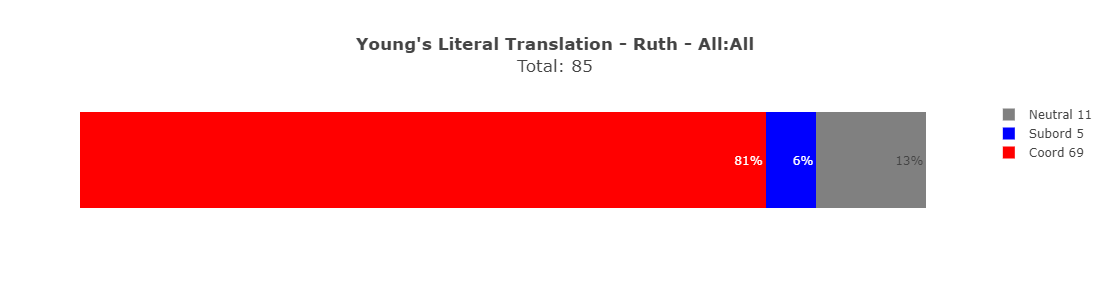
\includegraphics[width=1\linewidth]{template-komputasi-latex/YLT plots/bar YLT.png}
    \end{subfigure}
    \begin{subfigure}
       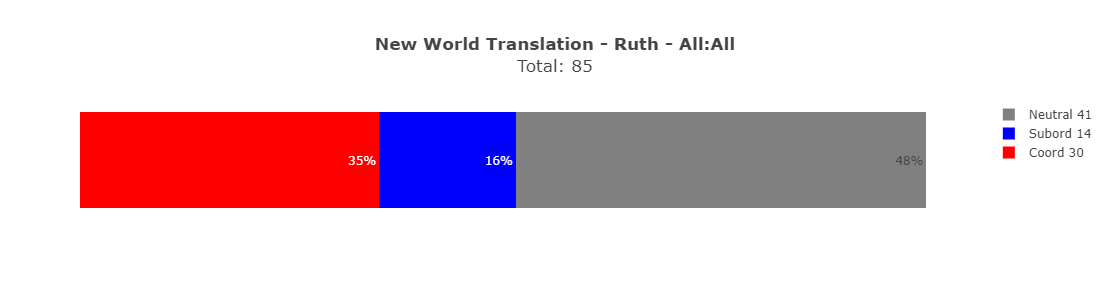
\includegraphics[width=1\linewidth]{template-komputasi-latex/NWT plots/bar NWT.png}
    \end{subfigure}
\caption{\label{fig:bar_comp} Bar plot comparison}
\end{figure}
As a preliminary inspection (Figure \ref{fig:bar_comp}), the user can clearly see the differences between the two versions of the book: the YLT is almost entirely made of coordinated sentences (81\%) with few verses being subordinated (6\%) or neutral (13\%); the NWT, on the other hand, has less than a half of coordinated sentences (35\%), more than the double of subordinated sentences (16\%) and it is composed mainly by neutral ones (48\%).

\subsection{Parallel Categories Diagram comparison}
\begin{figure}[!htpb]
    \centering
    \begin{subfigure}
       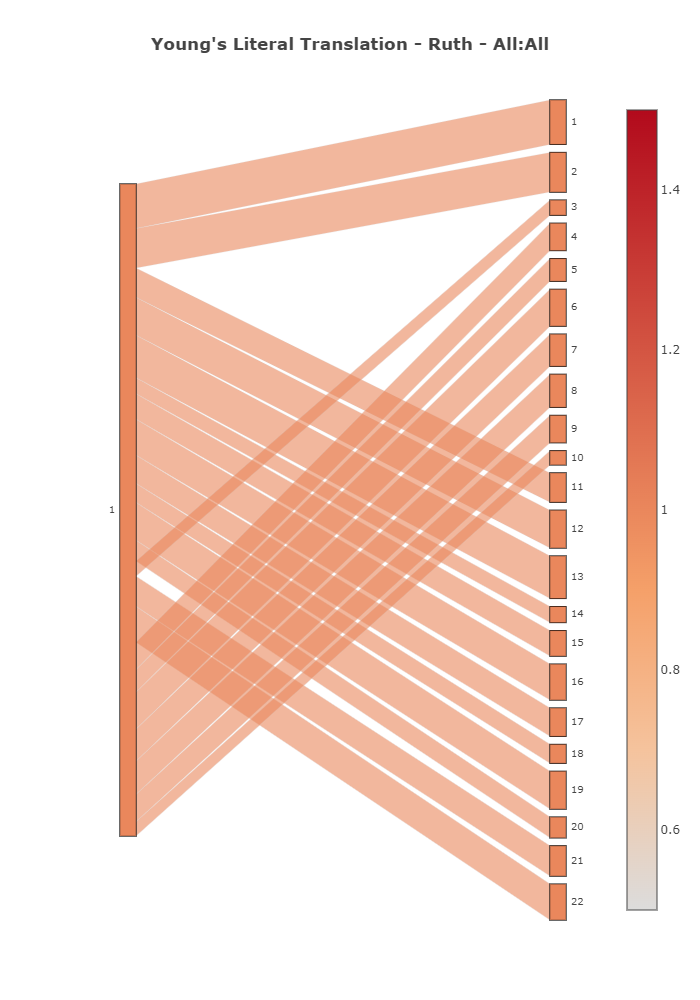
\includegraphics[width=0.4\linewidth]{template-komputasi-latex/YLT plots/catplot1 YLT.png}
    \end{subfigure}
    \begin{subfigure}
       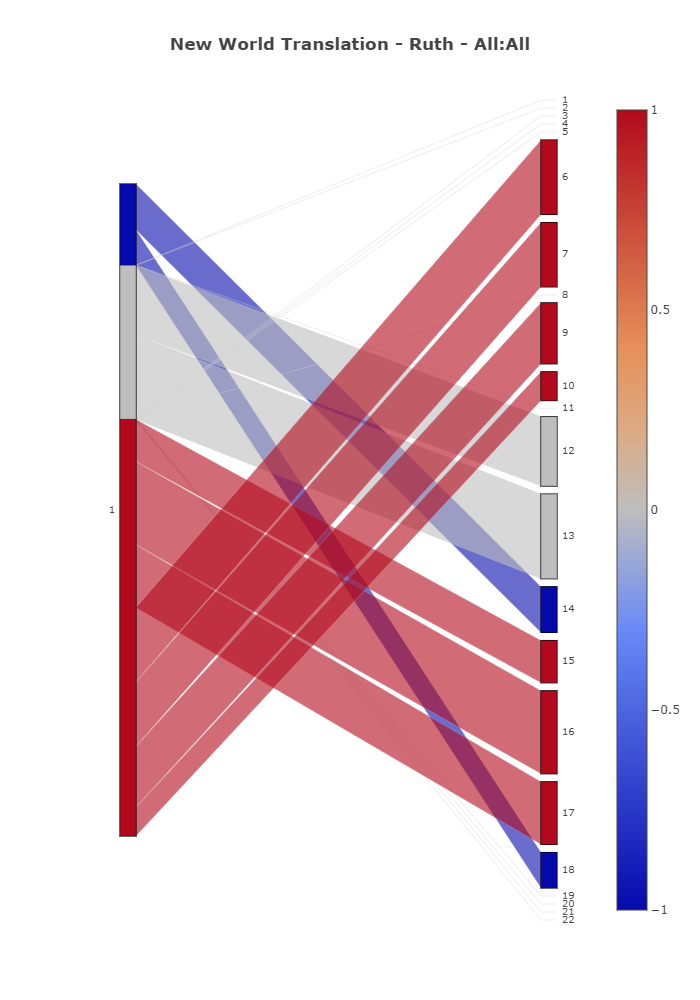
\includegraphics[width=0.4\linewidth]{template-komputasi-latex/NWT plots/catplot1 NWT.png}
    \end{subfigure}
\caption{\label{fig:catplot1_comp} Ruth's 1st chapter comparison}
\end{figure}
The first chapter of YLT version of Ruth book (Figure \ref{fig:catplot1_comp}) is entirely made by coordinated sentences. In NWT case, looking at the chapter axis: 64\% is made up of 64\% coordinated sentences, 12\% of subordinated ones and  24\% of neutral ones. Moreover,  11 verses are entirely omitted (1, 2, 3, 4, 5, 8, 11, 19, 20, 21, 22). An in-depth comparison of verses can be done using the apposite section. It is possible to notice a structure difference in verses 14,18, 11 and 12. \\ \\

\begin{figure}[!htpb]
    \centering
    \begin{subfigure}
       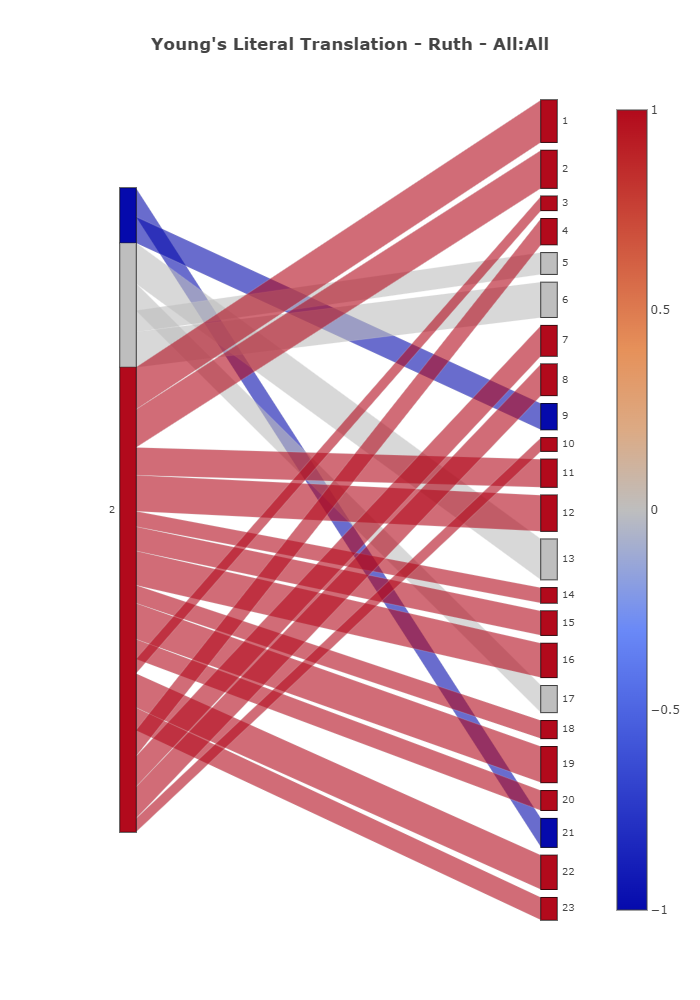
\includegraphics[width=0.4\linewidth]{template-komputasi-latex/YLT plots/catplot2 YLT.png}
    \end{subfigure}
    \begin{subfigure}
       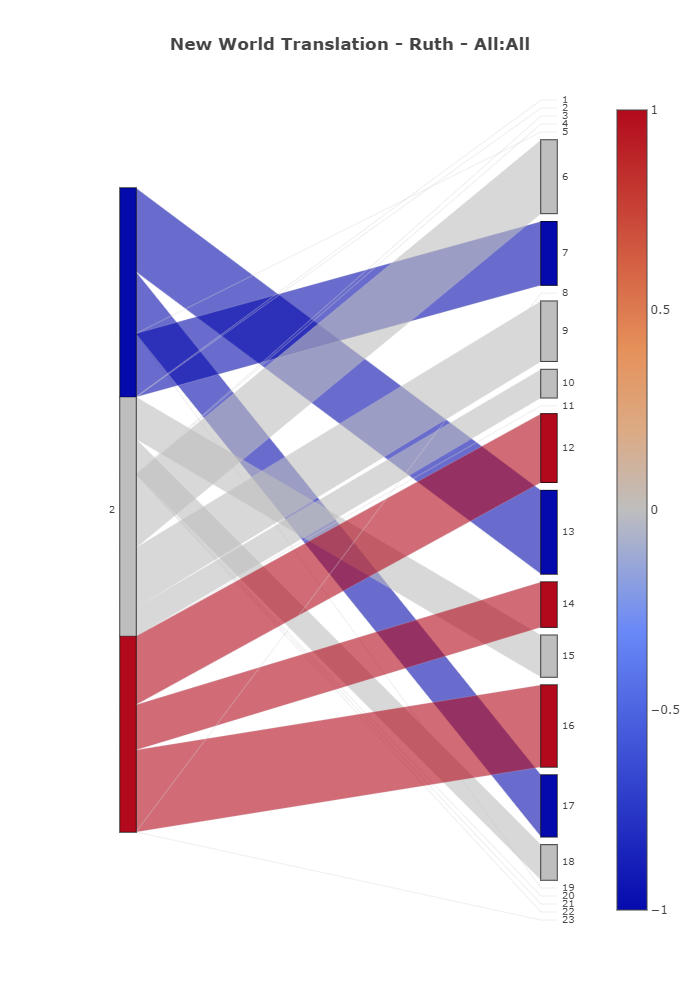
\includegraphics[width=0.4\linewidth]{template-komputasi-latex/NWT plots/catplot2 NWT.png}
    \end{subfigure}
\caption{\label{fig:catplot2_comp} Ruth's 2nd chapter comparison}
\end{figure}
In the case of the second chapter (Figure \ref{fig:catplot2_comp}), the YLT renders it as mostly coordinated (72\%) with a lesser part of subordinated (8\%, verses 9 and 21) and neutral (20\%, verses 5,6,13 and 17). In the NWT, on the other hand, the verses containing coordinated sentences are 30\%, the subordinated are 32\% (verses 7, 13 and 17) and the neutral ones are 38\% (verses 6, 9, 10, 15, 18). Again, there are omitted verses, 12 verses on a total of 23  (verses 1, 2, 3, 4, 5, 8, 11, 19, 20, 21, 22 and 23), basically almost 50\%. \\ \\

\begin{figure}[!htpb]
    \centering
    \begin{subfigure}
       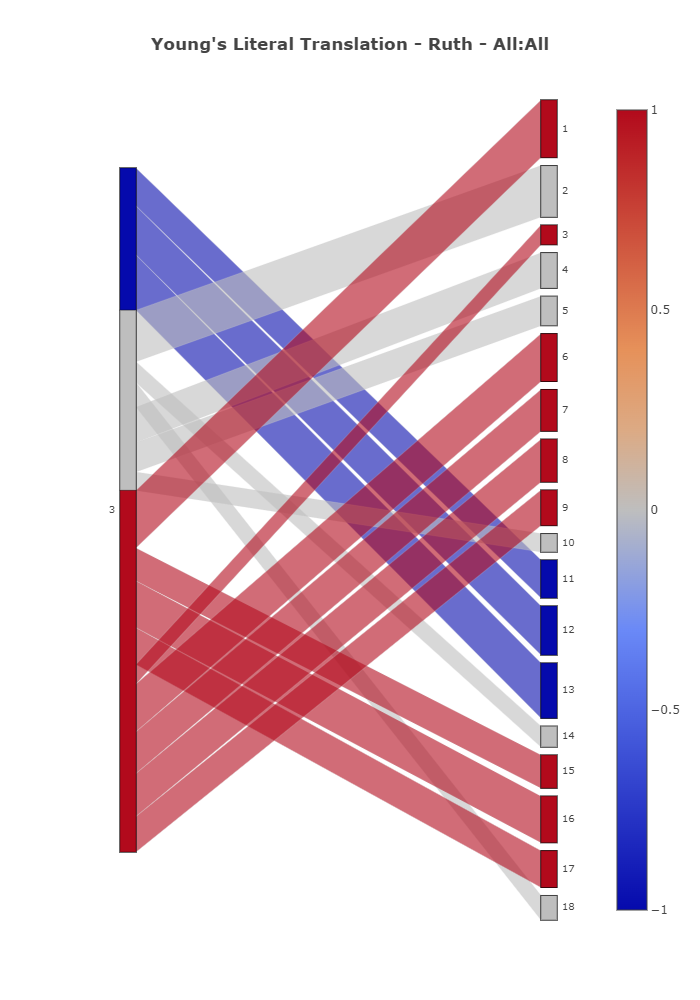
\includegraphics[width=0.4\linewidth]{template-komputasi-latex/YLT plots/catplot3 YLT.png}
    \end{subfigure}
    \begin{subfigure}
       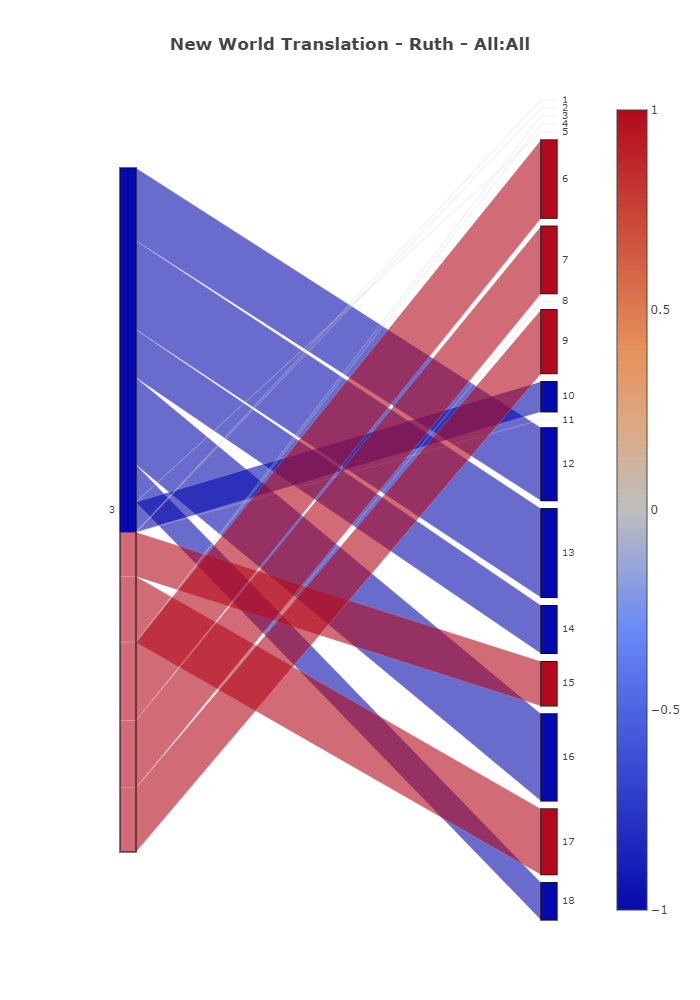
\includegraphics[width=0.4\linewidth]{template-komputasi-latex/NWT plots/catplot3 NWT.png}
    \end{subfigure}
\caption{\label{fig:catplot3_comp} Ruth's 3rd chapter comparison}
\end{figure}
In the case of the third chapter (Figure \ref{fig:catplot3_comp}), in YLT there are 53\% of coordinated sentences, 21\% of subordinated ones (verses 11, 12, 13) and 27\% of neutral ones (verses 2, 4, 5, 10, 14, 18). In the case of NWT it’s possible to see a clear difference: no neutral verses, but all coordinated (47\%) and subordinated ones (53\%, verses 10, 12, 13, 14, 16 and 18). Again, there are omitted verses: 1, 2, 3, 4, 5, 11. \\ \\

\begin{figure}[!htpb]
    \centering
    \begin{subfigure}
       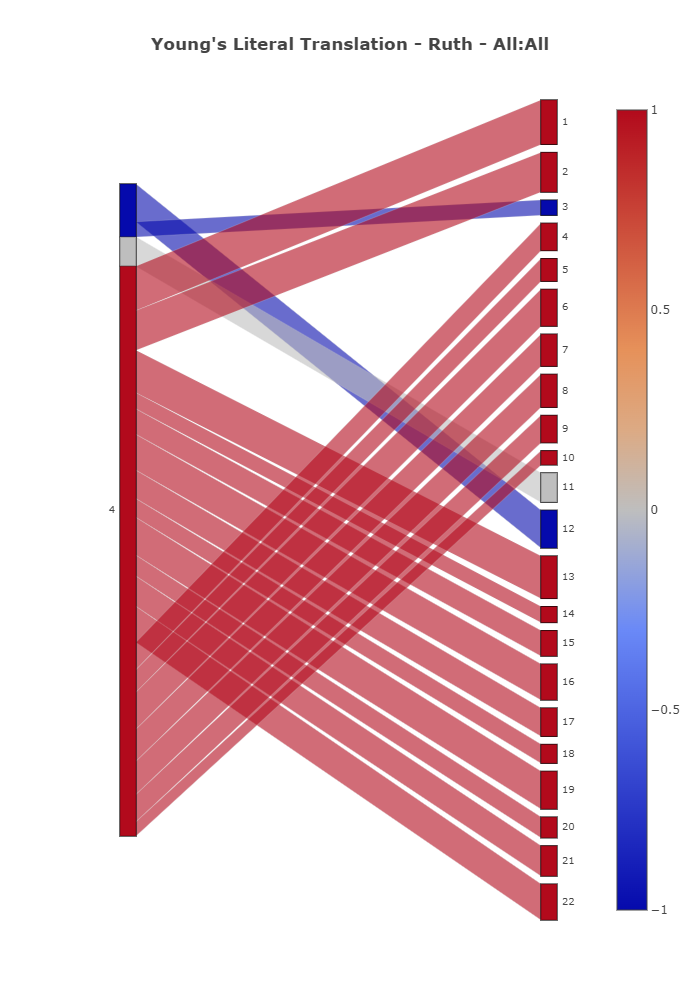
\includegraphics[width=0.4\linewidth]{template-komputasi-latex/YLT plots/catplot4 YLT.png}
    \end{subfigure}
    \begin{subfigure}
       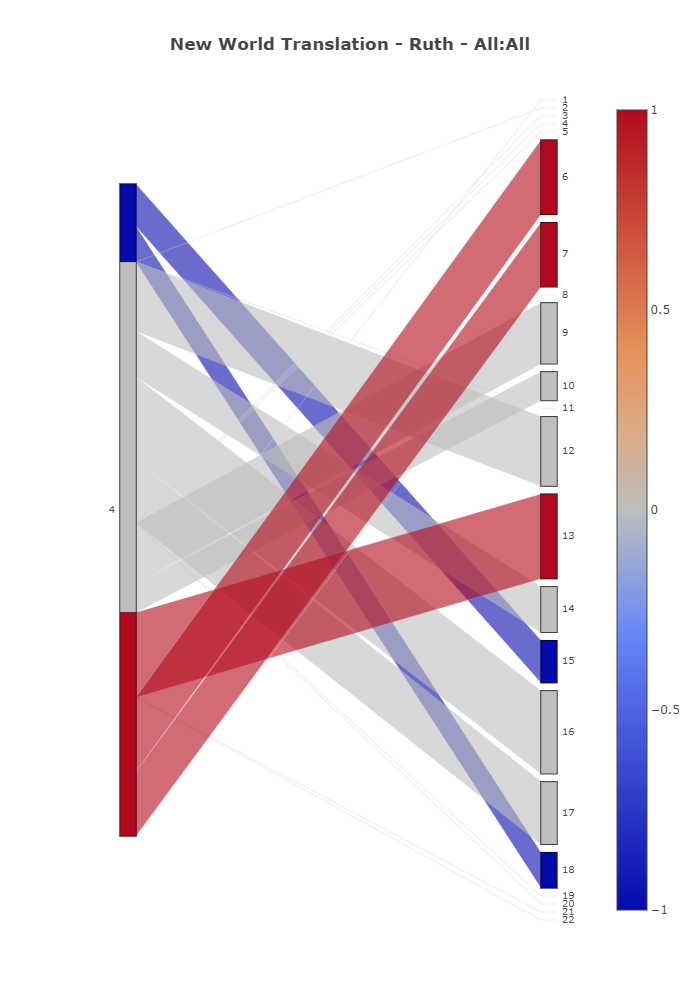
\includegraphics[width=0.4\linewidth]{template-komputasi-latex/NWT plots/catplot4 NWT.png}
    \end{subfigure}
\caption{\label{fig:catplot4_comp} Ruth's 4st chapter comparison}
\end{figure}
Finally, in the case of chapter 4 (Figure \ref{fig:catplot4_comp}), in YLT version it’s possible to notice that the vast majority of the verses are coordinated (88\%) and only a lesser percentage of subordinated (8\%, verses 3 and 12) and  neutral ones (4\%, only verse 11). On the other hand, in the NWT only the 34\% are coordinated, 12\% are subordinated (verses 15 and 18) and 54\% are neutral (verses 9, 10, 12, 14, 16 and 17). Again, 11 verses are omitted (verses 1, 2, 3, 4, 5, 8, 11, 19, 20, 21, 22): basically the 50\% of verses. \\ \\

Note that the effects of verse omissions  will be clearly visible in the network plot presented further.

\subsection{Line plot comparison}
\begin{figure}[!htpb]
    \centering
    \begin{subfigure}
       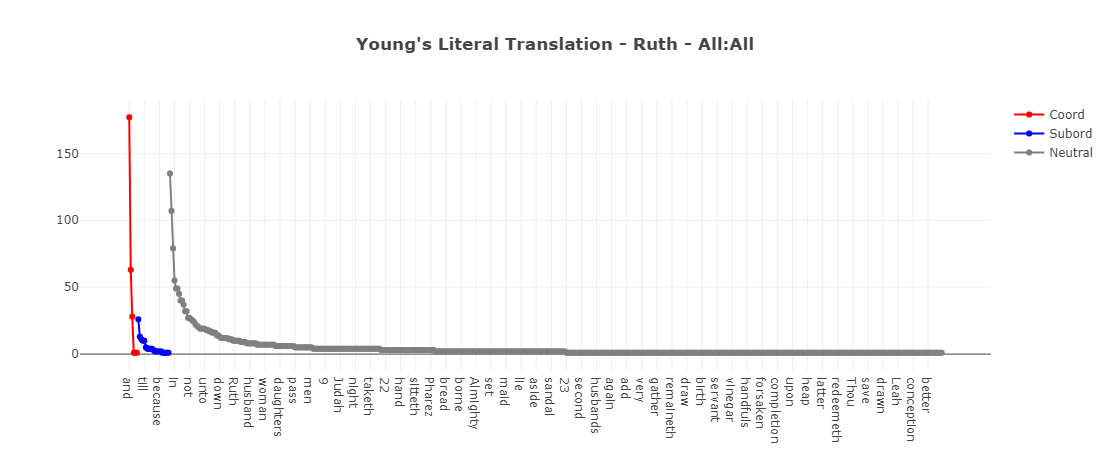
\includegraphics[width=1\linewidth]{template-komputasi-latex/YLT plots/line YLT.png}
    \end{subfigure}
    \begin{subfigure}
       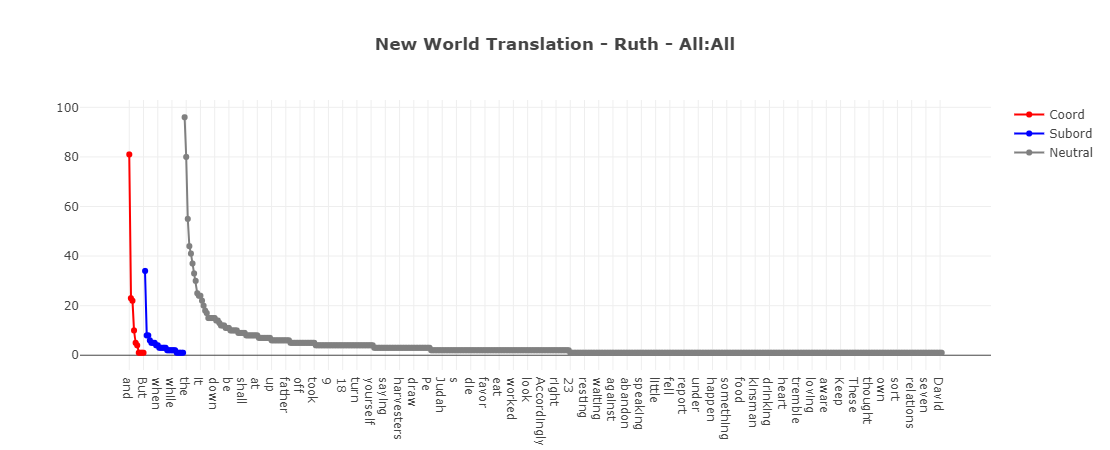
\includegraphics[width=1\linewidth]{template-komputasi-latex/NWT plots/line NWT.png}
    \end{subfigure}
\caption{\label{fig:line_comp} Line plot comparison}
\end{figure}
An inspection of each of the token would not be feasible in this context, so the most common ones are considered (Figure \ref{fig:line_comp}).
W.r.t to tokens, in the YLT case the most used token is the coordinating conjunction “and” (used 117 times) along with “And” (used 63 times). As already mentioned, the presence of the coordinating conjunction at the start of the sentences highlights a structure that clearly mirrors the juxtaposition of the orality (especially if repeatedly used at the beginning of the sentence, sentence after sentence). Generally, there is high presence of coordinating conjunctions compared to the subordinating ones ( the most used of these tokens is “that” with a frequency equal to 26, the same value of the third most frequent coordinating conjunction). By the way there is more heterogeneity in subordination usage (in the coordinated line there are just 3 highly used tokens, namely “and”, “And” and “for”, while the others are used only once).
By looking at the neutral line: “the” is the most used token  (135 times) followed by “to” (107 times), “of” (79 times) and “in” (55 times). 
In the NWT case, on the other hand, looking at the coordinate line: there is a major shrinkage of “and” usage (81 times) and the “And” usage (only 23 times) this time at the same level of “for” (the third most frequent coordinating conjunction). This would be enough to understand the shift happened in the translation: more than 40 sentences starting with “And” have been translated differently (or omitted), with an important loss at a structural level. By looking at the subordinated line, there are no major differences, aside from the higher usage of “that” (34 times) but a lower usage of other subordinating conjunctions. The other difference is noticeable in the neutral line: the first token in this case is “to” (96 times) followed by “the” (80 times), “you” (55 times) and “she” (44 times).  The swapping between “the” and “to” and their minor usage is sufficient to spot an important change in the structure of the sentences (aside from the discourse style).

\subsection{3D Scatterplot comparison}
\begin{figure}[!htpb]
    \centering
    \begin{subfigure}
       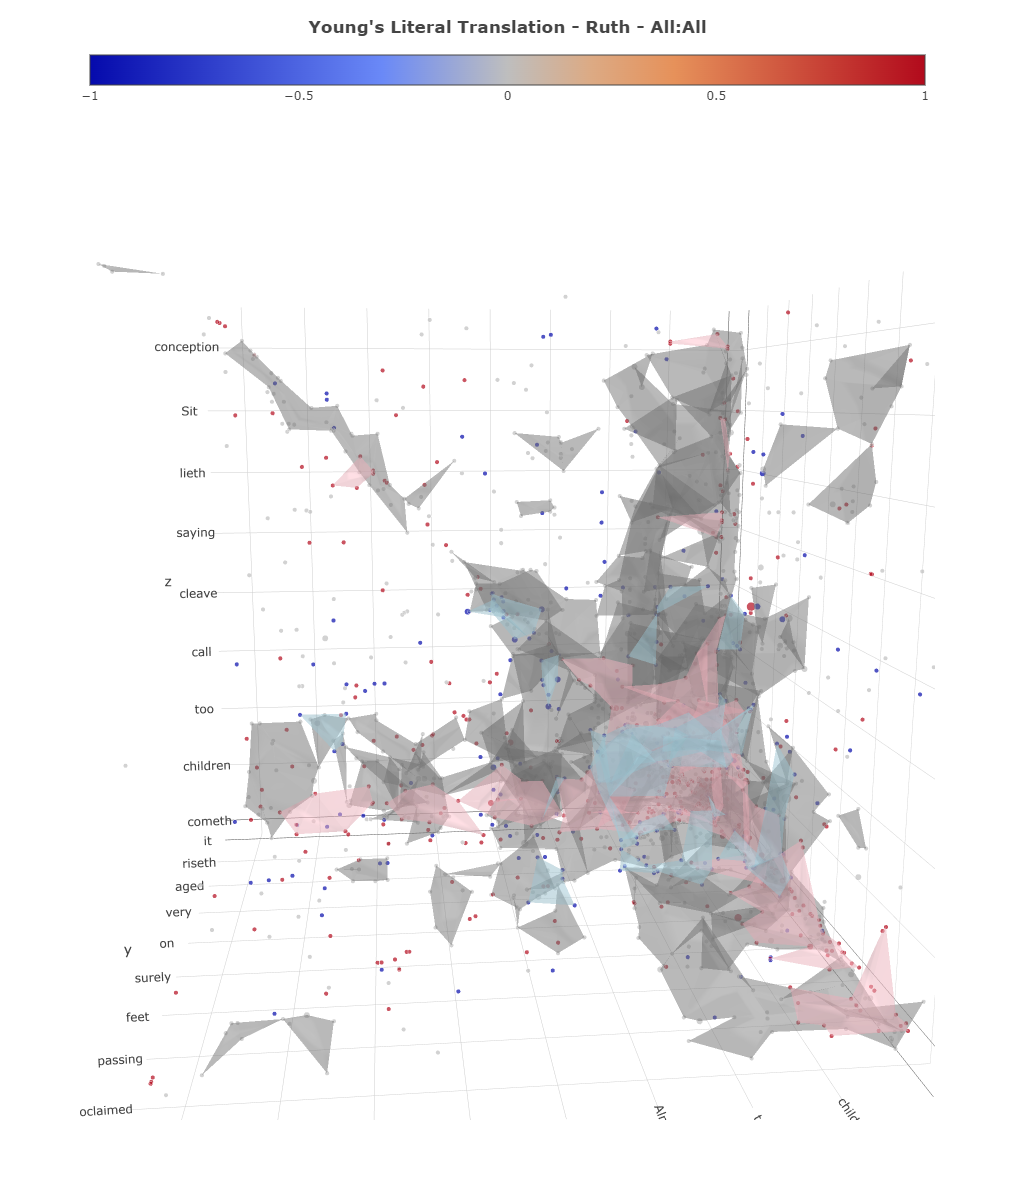
\includegraphics[scale=0.15]{template-komputasi-latex/YLT plots/scatter YLT.png}
    \end{subfigure}
    \begin{subfigure}
       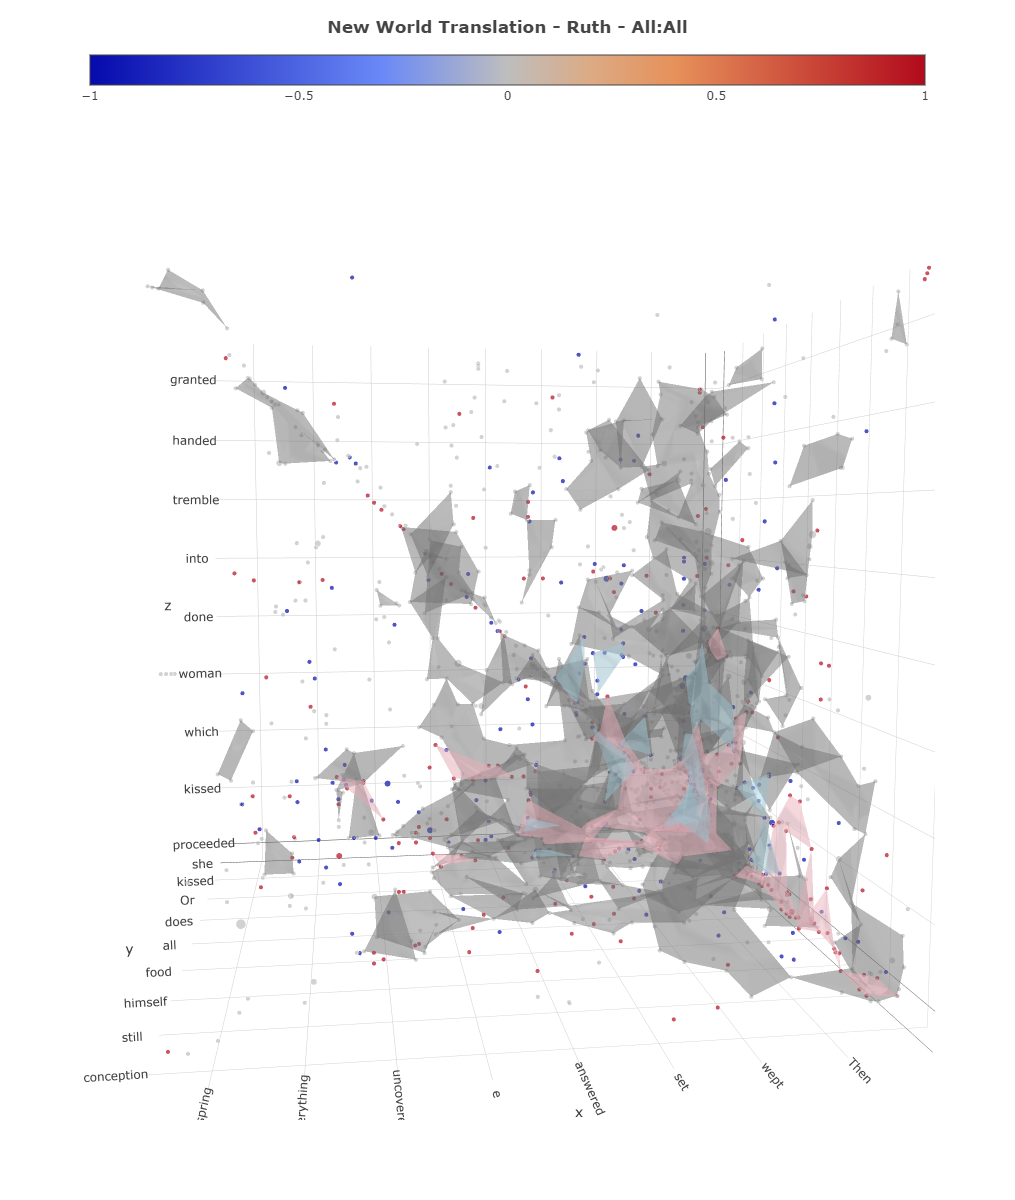
\includegraphics[scale=0.15]{template-komputasi-latex/NWT plots/scatter NWT.png}
    \end{subfigure}
\caption{\label{fig:scatter_comp} 3D Scatterplot comparison}
\end{figure}
Being a 3D plot, the analysis through interaction would be mandatory.  A brief yet absolutely not exhaustive description will be given by looking only at mesh layers (Figure \ref{fig:scatter_comp}). In this case, the triangulation highlights those portions of space having a high density of nodes. The parameter ruling the space occupied by the mesh (i.e. the number to consider sufficient to triangulate the space) is the “alphahull” parameter and the used value has been chosen inductively: a lower value would make the plot more cluttered than it already is (i.e. triangulating relatively low dense portions of space) and a higher value would reduce it too much. Note that lines drawn by nodes will not be considered cluster as they proceed in a linear fashion, fixed on a single axis (i.e trigrams having a fixed token in a fixed dimension, as in [‘you and I’, ‘house and the’, ‘high and low’] with a fixed y axis in this case). \\ \\

The first consideration in this case is that in the NWT, as has been shown, there are considerably less verses compared to YLT and thus less trigrams. This difference accounts for an unfair visual comparison as in YLT case it seems that there are more both trigrams with subordinating conjunctions or neutral ones but in reality there are more neutral trigrams in NWT (in percentage). A second consideration is that YLT seems more heterogeneous w.r.t trigram usage: the mesh is more diffused but again, this is consistent with the fact that YLT has more verses than NWT. 

The user is strongly invited to experiment with the plot and its selector. To replicate exactly the showed plot, the following values must be used in the selectors: Scaled values, Hide annotations, All, Apply mesh.

\subsection{Entity-Entity comparison}
Before proceeding note that colors in the heatmap stands for frequency and not for subordinate/coordinate distinction. \\ \\

\begin{figure}[!htpb]
    \centering
    \begin{subfigure}
       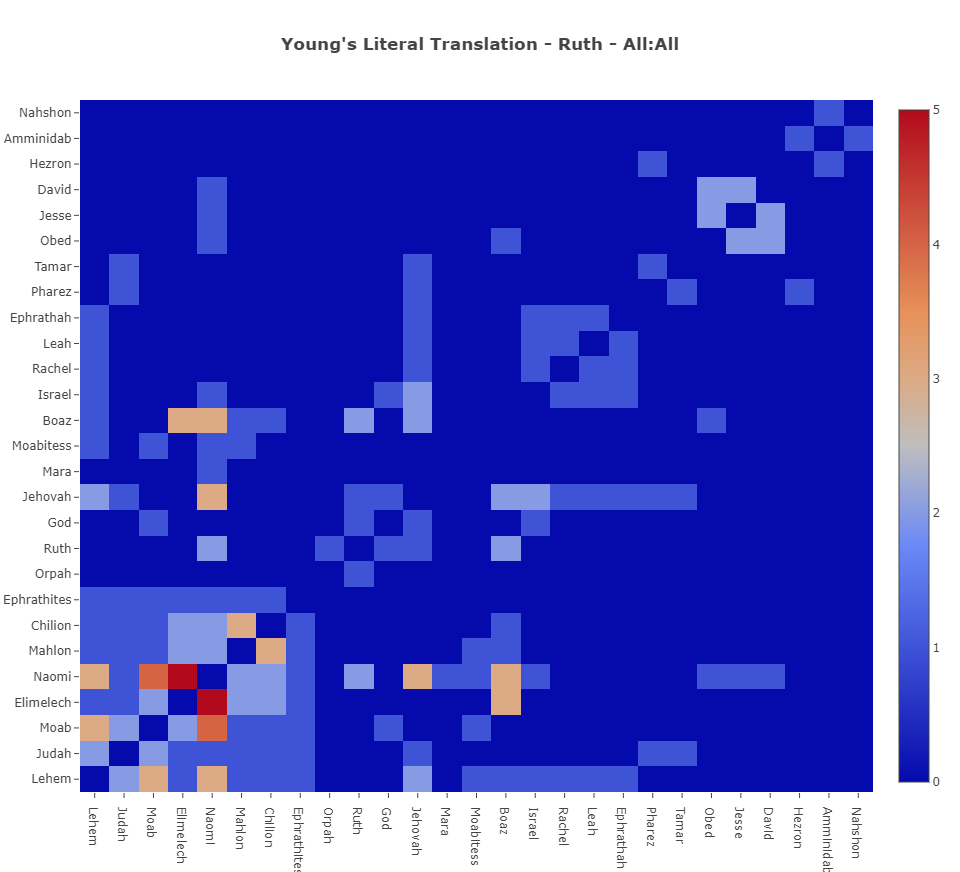
\includegraphics[scale=0.15]{template-komputasi-latex/YLT plots/entity-entity YLT.png}
    \end{subfigure}
    \begin{subfigure}
       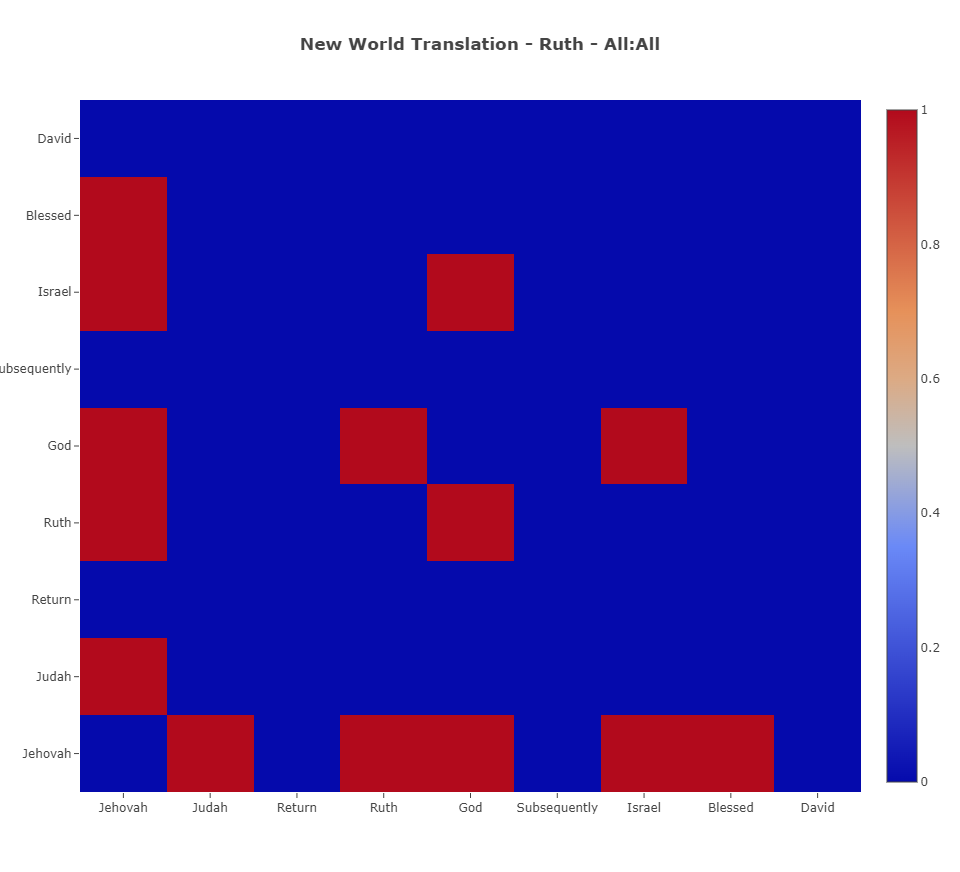
\includegraphics[scale=0.15]{template-komputasi-latex/NWT plots/entity-entity NWT.png}
    \end{subfigure}
\caption{\label{fig:entityentityheat_comp} Entity-Entity heatmap comparison}
\end{figure}
The first striking difference (Figure \ref{fig:entityentityheat_comp}), as already mentioned but more significantly visible, are the fewer names of NWT compared to YLT. Here it’s possible to understand the arbitrary selections of the Watch Tower (the head of Jeova’s witnesses) w.r.t verses: they are selected according to names. Ignoring lesser errors (like the presence of few common nouns) we can clearly see that they ignore the existence in the story of Lehem, Moab, Elimelech, Naomi, Mahlon, Boez and many others. Notice how these names (the firsts in the YLT heatmap except for Boez) are anything but irrelevant:
they seem to account actually for the core co-occurrence in the book, with Naomi-Elimelech being the most frequent one (5 times). In the NWT instead, every other co-occurrence is erased, leaving essentially: Judah, Ruth, God, Israel and David. \\ \\

In order to inspect also the sentiment tied to entities and context of co-occurrence, a network approach has been exploited (Figure \ref{fig:entityentitynetwork_comp}). Again, also this plot needs hover interaction to reach full informativity (i.e. by hovering or dragging the interested node to highlight its linked nodes) and colors here stand for sentiment, as explained at the beginning of the report.\\ \\

\begin{figure}[!htpb]
    \centering
    \begin{subfigure}
       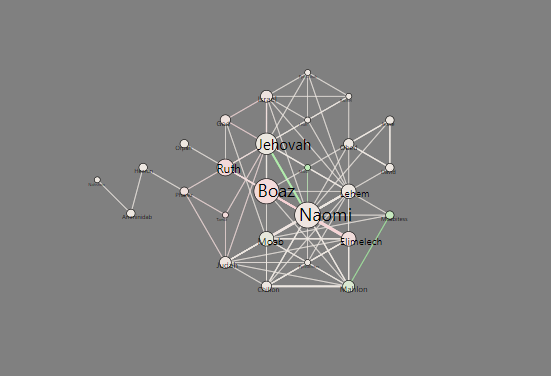
\includegraphics[scale=0.4]{template-komputasi-latex/YLT plots/network YLT.png}
    \end{subfigure}
    \begin{subfigure}
       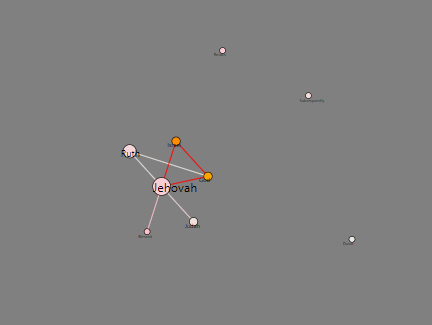
\includegraphics[scale=0.4]{template-komputasi-latex/NWT plots/network NWT.png}
    \end{subfigure}
\caption{\label{fig:entityentitynetwork_comp} Entity-Entity network comparison (YLT to the left; NWT to the right)}
\end{figure}
In the case of YLT it’s possible to notice that Naomi, Boaz, Jehovah, Ruth and Moab are the most frequent names. Maobites and Mahlon (both occurring in slightly negative contexts, -0.10 and -0.5) are tied mostly by negative contexts: this could mean that they both only appear in the same negative contexts (few contexts given the low width of the link). A more frequent negative link is that between Naomi and Jehovah but these two names appear in almost neutral contexts (0.01 and -0.01). Another negative bond is that between Naomi and Mara (a name appearing only once, in -0.13 context). Finally the strongest ties of the network are that of Naomi with Elimelech, Moab, Lehem, Jehovah and Boaz. The user is invited to explore more in depth the co-occurence of names and their indirect connections (e.g. Mahlon connects to Naomi that connects to Jehovah) among other things. An example of selection feature is displayed in Figure \ref{fig:network_selection}.
\begin{figure}[!htpb]
    \centering
    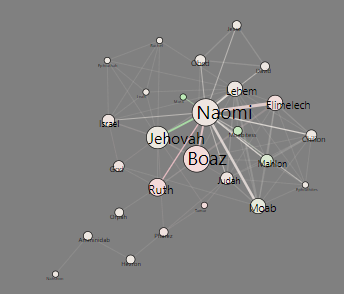
\includegraphics[scale=0.5]{template-komputasi-latex/YLT plots/network selection YLT.png}
    \caption{Network selection feature}
    \label{fig:network_selection}
\end{figure} \\ \\

In the case of NWT now more clearly appears the effect of this kind of censorship: entire set of entities and contexts are purposely omitted, led by the need of ideology.
Only Jehovah, Ruth, Israel, God and David remain, with a strongly positive link between Jehovah, God and Israel and no negative links or contexts. Considering that the YLT is an attempt to be radically close to the original writings, that of the Watch Tower in the NWT is a deep and intellectually dishonest text manipulation.

\subsection{Entity-Summary comparison}
\begin{figure}[!htpb]
    \centering
    \begin{subfigure}
       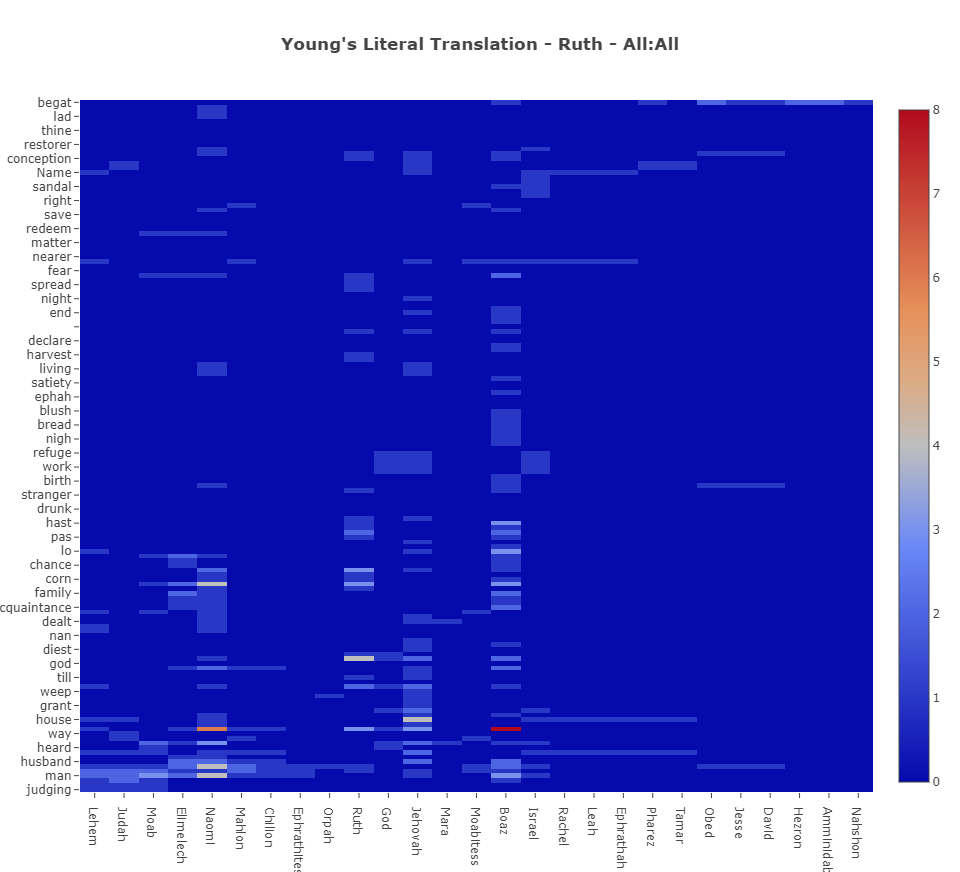
\includegraphics[scale=0.15]{template-komputasi-latex/YLT plots/entity-summary YLT.png}
    \end{subfigure}
    \begin{subfigure}
       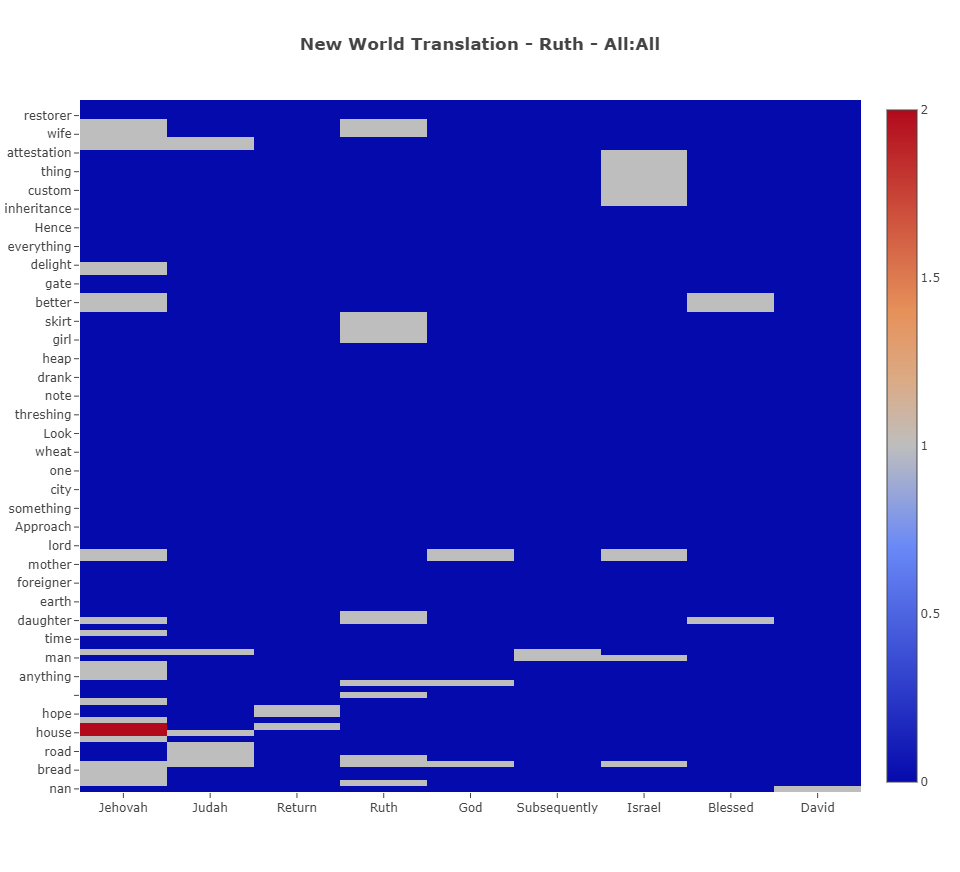
\includegraphics[scale=0.15]{template-komputasi-latex/NWT plots/entity-summary NWT.png}
    \end{subfigure}
\caption{\label{fig:entitysummaryheat_comp} Entity-Summary heatmap comparison}
\end{figure}
In the YLT heatmap (Figure \ref{fig:entitysummaryheat_comp}), “Boaz-saith” is the most frequent occurrence (8 times) along with “Naomi-saith”. This is significant as the repetition of a pattern, in particular something that precedes a direct discourse, is a strong sign of orality. Limiting the observation to Naomi and  Boaz, we can say that Boaz appears continuously during the narration while Naomi almost disappears at half of the narration. Notice that “Jehovah-house” appears only 4 times (half less than “Boaz-saith”).
In the NWT version, the most frequent co-occurrence is “Jehovah-house” as well as “Jehovah-husband” (4 times) anything else appear only once. Further things could be said about the semantics of the co-occurrence but it’s not the aim of the present project. The user is strongly suggested to use the plot interactively (as ticks label are only partially visible) to inspect and spot significant patterns.

\section{Conclusions?}
As previously mentioned in the introduction, there is no conclusion. It is an open-posed problem. It could be reasonably said, based on Ruth book, that NWT version seems to be radically manipulated by the mean of ideology. This conclusion could be drawn certainly by inspecting book by book as done in this work or better, by accessing more information through interaction. This project is conceived to be a potentially scalable analysis tool for bible versions. The user is called to draw the conclusions.

\bibliographystyle{ACM-Reference-Format}
\bibliography{biblio}
\end{document}
